\documentclass[11pt]{article}

%%
%% PACKAGES
%%

\usepackage[letterpaper, includeheadfoot, margin=0.9in,top=0.7in,bottom=0.8in]{geometry}
\usepackage[charter]{mathdesign} % Main font
\usepackage[scaled]{beramono} % Lovely monospace font
\usepackage[T1]{fontenc}
%\usepackage{amsmath, amssymb}
\usepackage{bm}
\usepackage{mathtools}
\usepackage{mathdots}
\usepackage{titlesec} % Custom section headings.
\usepackage{microtype}
\usepackage{xcolor}
\usepackage{xspace}
\usepackage{xfrac}
\usepackage{calc}
\usepackage{outlines}
\usepackage{natbib}

% Graphics.
%\usepackage{graphicx}
\usepackage{overpic}
\usepackage[update,prepend]{epstopdf} % To use eps files.

% Code listings.
\usepackage{listings} % Code listings.
\usepackage{matlab-prettifier} % MATLAB code listings

% Tweaks for captions and enumerations.
\usepackage[labelfont=bf]{caption} % Figure captions.
\usepackage{enumitem} % Fine tuning enumerations.
%\usepackage{floatrow} % Captions to the right of figures.

% Plotting and drawing
\usepackage{tikz} % This automatically loads graphicx!
\usetikzlibrary{calc} % For relative positions to defined coords
\usepackage{pgfplots} % Scientific plotting tools
\pgfplotsset{compat=1.7}

% Figure placement
%\usepackage{wrapfig}
%\captionsetup[wrapfigure]{margin=0.5cm}

% Packages to makes tables pretty.
\usepackage{array}
\usepackage{booktabs}
\setlength{\heavyrulewidth}{1.5pt}
\setlength{\abovetopsep}{4pt}
\renewcommand{\arraystretch}{1.2}

% Fancyhdr package stuff...
\usepackage{fancyhdr}
\setlength{\headheight}{30pt}
%\renewcommand{\headrulewidth}{0pt}
%\renewcommand{\footrulewidth}{0pt}

%%
%% SETTINGS
%%

% Path to look for graphics
\graphicspath{{../images/}}
%\epstopdfsetup{outdir=../images/}

% Caption spacing
\setlength{\abovecaptionskip}{0pt}

% List spacing
\setlist{noitemsep}

% Math operator font
\DeclareSymbolFont{sfoperators}{OT1}{cmss}{m}{n}
\DeclareSymbolFontAlphabet{\mathsf}{sfoperators}
\makeatletter
\def\operator@font{\mathgroup\symsfoperators}
\makeatother

%% No indent all paragraphs
%\setlength{\parindent}{0in}

% Figure references
\newcommand{\figref}[1]{Figure~\ref{#1}}

% Special format section headings
\titleformat{\section}%
	{\large\bf\scshape}% Text formatting
	{\arabic{section}}% Number
	{1em}% Space between number and text
	{}% Code before
	[]% Code after
\titleformat{\subsection}%
	{\normalsize\bf\scshape}% Text formatting
	{\arabic{section}.\arabic{subsection}}% Number
	{1em}% Space between number and text
	{}% Code before
	[]% Code after
%\titleformat{\subsubsection}%
%	{\color{blue}}% Text formatting
%	{\arabic{subsubsection} $\rightarrow$}% Number
%	{1em}% Space between number and text
%	{}% Code before
%	[]% Code after

%\definecolor{mygray}{rgb}{0.4, 0.4, 0.4}
%\lstset{
%style=Matlab-editor,
%mlscaleinline=false,
%basicstyle=\ttfamily\lst@ifdisplaystyle\scriptsize\fi,
%frame=single,
%rulecolor=\color{mygray},
%numbers=left,
%numbersep=10pt,
%numberstyle=\footnotesize \ttfamily \color{mygray},
%xleftmargin=30pt,
%xrightmargin=5pt,
%framexleftmargin=4pt,
%framextopmargin=2pt
%}
\lstset{
basicstyle=\ttfamily
}

% Allow white-space to be eaten within any lst environments between returns.
\lstset{breaklines,breakatwhitespace}

% Define a chacacter as shorthand for inline listings.
\lstMakeShortInline[basicstyle=\color{cyan!60!black}\small]{|}

%%
%% COMMANDS
%%

% Various plot lines to include in-line.
\newcommand{\solidrule}[1][8mm]{\rule[0.5ex]{#1}{1.5pt}}
\newcommand{\dashrule}{\mbox{%
	\solidrule[2mm]\hspace{1mm}\solidrule[2mm]\hspace{1mm}\solidrule[2mm]}}
\newcommand{\dotdashrule}{\mbox{%
	\solidrule[0.5mm]\hspace{1mm}\solidrule[2mm]\hspace{1mm}\solidrule[0.5mm]\hspace{1mm}\solidrule[2mm]}}

% Automated file inclusion for code listings
\makeatletter
\def\includecode{\@ifnextchar[{\@with}{\@without}}
\def\@with[#1]#2{
}
\def\@without#1{
  \lstinputlisting[caption=\ttfamily\protect\detokenize{#1}, escapechar=, frame=single]{../matlab_code/#1}
}
\makeatother

% Degree symbol.
\newcommand{\degree}{\ensuremath{^\circ}}

% Superscript text: 1st, 2nd, 3rd, 4th
\newcommand{\suptext}[1]{\ensuremath{^\text{#1}}\xspace}
\newcommand{\st}{\suptext{st}}
\newcommand{\nd}{\suptext{nd}}
\newcommand{\rd}{\suptext{rd}}
\let\oldth\th % Reassign the current \th command
\renewcommand{\th}{\suptext{th}}

% Underline matrices
\newcommand{\ul}[1]{\smash{\underline{#1}}}
\newcommand{\uul}[1]{\smash{\underline{\underline{#1}}}}

% Partial derivatives
\newcommand{\pp}[2]{\ensuremath{\frac{\partial#1}{\partial#2}}}

% Error function
\DeclareMathOperator\erf{erf}

% Big O notation
\newcommand{\bigo}{\ensuremath{\mathcal{O}}}

% Citation flag
\newcommand{\citeme}{{\color{red}\textbf{[cite]}}}

% Derivatives
\newcommand{\dd}[2]{\ensuremath{\frac{d #1}{d #2}}}
\newcommand{\pdd}[2]{\ensuremath{\frac{\partial #1}{\partial #2}}}
\newcommand{\tdd}[2]{\ensuremath{d #1 / d #2}}
\newcommand{\tpdd}[2]{\ensuremath{\partial #1 / \partial #2}}

% Text max and min
\newcommand{\tmax}{\ensuremath{\text{max}}}
\newcommand{\tmin}{\ensuremath{\text{min}}}

% Norm
\newcommand{\norm}[1]{\ensuremath{\left| #1 \right|}}

% Bold vectors
% Option 1: Works on more than single tokens, but makes regular letters italic as well as bold.
%\renewcommand{\vec}[1]{\mathbold{#1}}
% Option 2: Only works if a single token is passed to the command, but makes regular letters bold only.
\newcommand{\mb}[1]{
	\ifcat\noexpand#1\relax
		\expandafter\mathbold
	\else
		\expandafter\mathbf
	\fi{{#1}}
}

% Underlines for tensor notation.
\newcommand{\tsr}[1]{\ensuremath{\underline{#1}}}
\newcommand{\tsrr}[1]{\ensuremath{\underline{\underline{#1}}}}

% Allow lstinline within math mode. At bottom of this file b/c of syntax highlighting.
%\usepackage{letltxmacro}
%\newcommand*{\SavedLstInline}{}
%\LetLtxMacro\SavedLstInline\lstinline
%\DeclareRobustCommand*{\lstinline}{%
%  \ifmmode
%    \let\SavedBGroup\bgroup
%    \def\bgroup{%
%      \let\bgroup\SavedBGroup
%      \hbox\bgroup
%    }%
%  \fi
%  \SavedLstInline
%}


%%
%% DOCUMENT START
%%

\begin{document}
\fancypagestyle{allpages}
{
	\fancyhf[LH]{Bi-Fidelity Modeling of a NACA Airfoil}
	\fancyhf[CH]{}
	\fancyhf[RH]{\thepage}
	\fancyhf[LF]{}
	\fancyhf[CF]{}
	\fancyhf[RF]{}
}

\fancypagestyle{firstpage}
{
	\fancyhf[LH]{\Large Final Project \\ \large ASEN 6519: Uncertainty Quantification}
	\fancyhf[CH]{}
	\fancyhf[RH]{\large Ryan Skinner \\ \large Due 2016/5/6}
	\fancyhf[LF]{}
	\fancyhf[CF]{}
	\fancyhf[RF]{}
}

\pagestyle{allpages}
\thispagestyle{firstpage}
\renewcommand{\sectionmark}[1]{ \markright{#1}{} }

\vspace*{0in}
\begin{center}
\Large
Bi-Fidelity Modeling of Geometric Impact on NACA Airfoil Performance
\\[1ex]
\large
Ryan Skinner$^1$
\\[1ex]
\normalsize
$^1$University of Colorado, Boulder, CO USA
\end{center}

\section*{Abstract}
This bi-fidelity investigation explores the effect of variation in geometry and angle of attack on the performance of a 2-D NACA 4412 airfoil. The flow is incompressible and is characterized by a Reynolds number of 3 million. All simulations are steady and rely on the Spalart-Allmaras (SA) RANS turbulence closure. Low-fidelity simulations use a coarse mesh with unresolved boundary layers (BLs), whereas high-fidelity simulations employ a refined mesh that fully resolves the near-wall BL. Predictive capacity of the bi-fidelity approach is analysed with pressure coefficient data.

%%%%%%%%%%%%%%%%%%%%%%%%%%%%%%%%%%%%%%%%%
%%%%%%%%%%%%%%%%%%%%%%%%%%%%%%%%%%%%%%%%%
\section{Introduction and Motivation}
%%%%%%%%%%%%%%%%%%%%%%%%%%%%%%%%%%%%%%%%%
%%%%%%%%%%%%%%%%%%%%%%%%%%%%%%%%%%%%%%%%%

The need to characterize and optimize the design of unsteady aerodynamic systems becomes more pressing as atmospheric vehicles push performance boundaries. Despite advances over the last five decades in turbulence modeling, accurately capturing the dynamics critical to these systems is computationally expensive. In most cases, this expense precludes thorough uncertainty quantification (UQ) and design optimization (DO) of the system. Accordingly, the finite time to market for most high-performance aerospace products constrains simulations' quantity and rigor, and can lead to uncertain and sub-optimal performance. Any method that ameliorates this problem is directly applicable to industry.

The bi-fidelity approach seeks to address the shortcomings of traditional brute-force UQ/DO strategies. Bi-fidelity modeling has two steps. First, a number of low-fidelity (LF) simulations are run. LF simulations do not capture the exact physics of the system, but place low demand on computational resources. These LF realizations are used to generate both an interpolation and a low-rank approximation of a solution quantity as a function of design parameters. For aerodynamics, LF simulations may employ less stringent numerical convergence criteria, coarser meshes, or less-accurate turbulence models. Second, high-fidelity (HF) simulations are run for each combination of parameters deemed important by the low-rank approximation. HF simulations are ideally as accurate as possible, addressing all shortcomings of the LF model. The HF results are used in conjunction with the low-fidelity interpolating coefficients to approximate the solution response over the parameter space.

The present work seeks to quantify the effect of variability in geometric parameters defining a NACA 4-digit series airfoil on the $C_p$ distribution across its surface. Though 2-D NACA airfoils command little topical interest, this family is nonetheless selected for two reasons. First, it is a standard academic geometry that was thoroughly studied in the 1930s and '40s, resulting in readily-available validation data \citeme. Second, applying the bi-fidelity approach to a NACA airfoil offers a proving ground for the method and analysis tools, which can be scaled up to more industrially-relevant systems in future work. Ultimately, this technology will be extended to multi-fidelity simulations of flow over complex engineering geometries characterized by highly-unsteady separation. Such examples could include a multi-element airfoil at high-$\alpha$ or active flow control in an aggressive subsonic diffuser.

%%%%%%%%%%%%%%%%%%%%%%%%%%%%%%%%%%%%%%%%%
%%%%%%%%%%%%%%%%%%%%%%%%%%%%%%%%%%%%%%%%%
\section{Solution Approach}
%%%%%%%%%%%%%%%%%%%%%%%%%%%%%%%%%%%%%%%%%
%%%%%%%%%%%%%%%%%%%%%%%%%%%%%%%%%%%%%%%%%

\subsection{NACA 4-Digit Airfoils}

Before discussing simulation and bi-fidelity modeling details, it is fitting to quantify the geometry under study. The shape of a NACA 4-digit airfoil is defined by its maximum camber $m$, location of maximum camber $p$, maximum thickness $t$. These are non-dimensionalized by the airfoil chord $c$, which we take to be unity. We also consider the angle of attack $\alpha$ as a geometric parameter.

\begin{figure}[b]
\begin{center}
\includegraphics[width=0.6\textwidth]{example_deformation.eps}
\\[1ex]
\caption{Deforming a NACA 0012 airfoil ({\color{red}red}) to an arbitrary NACA 4-digit airfoil ({\color{blue}blue}). Point displacements indicated in black.}
\label{fig:naca_deform}
\end{center}
\end{figure}

The thickness of a symmetric airfoil corresponding to the NACA 00xx series is given by
\begin{equation}
y_t = 5tc\, \left[ 0.2969 \sqrt{\frac{x}{c}} + (-0.1260) \left(\frac{x}{c}\right) + (-0.3516) \left(\frac{x}{c}\right)^2 + 0.2843 \left(\frac{x}{c}\right)^3 + (-0.1015) \left( \frac{x}{c} \right)^4 \right]
\end{equation}
where $x \in [0, c]$ is a physical coordinate in the stream-wise direction. The coordinate pairs of points on the upper $(x_U, y_U)$ and lower $(x_L, y_L)$ surfaces are simply $x_U = x_L = x$, $y_U = y_t$, and $y_L = -y_t$. An example of the NACA 0012 airfoil is shown in Figure \ref{fig:naca_deform}.

Cambered NACA airfoils define thickness perpendicular to the camber line, which is given by
\begin{equation}
y_c = \begin{cases}
m \frac{x}{p^2} \left( 2p-\frac{x}{c}\right) & 0 \le x \le pc \\
m \frac{c-x}{(1-p)^2} \left(1-2p+\frac{x}{c}\right) & pc \le x \le c
\end{cases}
\end{equation}
Accounting for camber, the upper and lower coordinate pairs become
\begin{equation}
\begin{aligned}
x_U &= x - y_t \sin \theta &\quad y_U &= y_c + y_t \cos \theta \\
x_L &= x + y_t \sin \theta &\quad y_L &= y_c - y_t \cos \theta
\end{aligned}
\end{equation}
where
\begin{equation}
\theta = \arctan \left( \dd{y_c}{x} \right)
\quad \text{and} \quad
\dd{y_c}{x} =
\begin{cases}
\frac{2m}{p^2} \left( p - \frac{x}{c} \right) & 0 \le x \le pc \\
\frac{2m}{(1-p)^2} \left( p - \frac{x}{c} \right) & pc \le x \le c
\end{cases}
\end{equation}

Because cambered profiles are generated from their symmetric counterparts, we can analytically determine the displacements necessary to deform any volume (in our case, that around a NACA 0012 airfoil) into an arbitrary 4-digit NACA mesh. Figure \ref{fig:naca_deform} illustrates this concept. As will be explained later, this ability results in substantial efficiency gains when running multiple simulations of different geometries.

\subsection{Flow Simulation}

\begin{figure}[t]
\begin{center}
\begin{overpic}[width=\textwidth]{domain_grid.png}
	\put (3, 13.5) {\small \parbox[t][2in][t]{2in}{\emph{Inflow}\\
									 $u_{(x,y,x)}=(120,0,0)$ m/s\\
									 $T = 273.15$ K\\
									 $\nu_T = 0.0027$ m$^2$/s}}
	\put (30,13.5) {\small \parbox[t][2in][t]{2in}{\emph{Wing}\\
									 no-slip\\
									 $\nu_T = 0$\\
									 $T = 273.15$ K}}
	\put (45,13.5) {\small \parbox[t][2in][t]{2in}{\emph{Top/Bottom}\\
									 no-pen\\
									 $T = 273.15$ K}}
	\put (62,13.5) {\small \parbox[t][2in][t]{2in}{\emph{Front/Back}\\
									 no-pen\\
									 heat flux zero\\
									 $\nu_T$ flux zero}}
	\put (80,13.5) {\small \parbox[t][2in][t]{2in}{\emph{Outflow}\\
									 heat flux zero\\
									 traction vector zero\\
									 $p = 1\times 10^5$ Pa}}
\end{overpic}
\\[1.5ex]
\caption{Schematic of computational domain with BCs listed. Spatial units in meters.}
\label{fig:domain}
\end{center}
\end{figure}

Simulations are run in PHASTA, the parallel hierarchic adaptive stabilized transient analysis CFD code developed and maintained by Prof. Kenneth Jansen's group at the University of Colorado at Boulder. The compressible branch is used solely to carry out the mesh deformation, and the incompressible branch is used to actually run the simulation. The lack of PETSc integration in the incompressible formulation necessitates this somewhat disjointed workflow.

A schematic of the computational fluid domain is shown in Figure \ref{fig:domain}. It has streamwise length $L = 60$~m, vertical height $H = 10$~m, and span-wise width $W = 0.01$~m. These dimensions correspond to Cartesian directions $x$, $y$, and $z$ respectively. The airfoil's chord is $1.0$~m, and its leading edge is located $15$~m upstream from the inflow and equidistant from the top and bottom walls.

Simulations are incompressible, target a Reynolds number of 3 million with respect to the airfoil chord, and use the Spalart-Allmaras (SA) RANS turbulence closure. The fluid has a density of $\rho = 1.0$~kg/m$^3$ and a kinematic viscosity of $4.0 \times 10^{-5}$~m$^2$/s. Fluid enters the domain from the $-x$ face with a velocity of $120$~m/s in the $+x$-direction. The airfoil has no-slip boundary conditions applied. All faces have an essential temperature BC set to $273.15$~K, except for the $\pm z$ sidewalls and $+x$ outflow, which set natural temperature flux to zero. The outflow's essential pressure is set to $1\times 10^{5}$~Pa. The $\pm y$ and $\pm z$ walls are inviscid and impenetrable.

To seek a steady solution, both LF and HF simulations are run at a fairly large time step of $\Delta t = 1 \times 10^{-2}$~s with first-order time integration until negligible solution change is observed between iterations, and the flow and SA turbulence scalar absolute errors drop below $2 \times 10^{-3}$ and $2 \times 10^{-5}$, respectively. Meeting this criterion typically requires between 30 and 50 time steps.

\subsection{Mesh Generation}

For both the LF and HF runs, we begin by meshing the fluid volume around a standard NACA 0012 airfoil at zero angle of attack, the outline of which is shown in Figure \ref{fig:naca_deform}. This allows us to iterate the mesh until it adequately captures the curvature of this family of airfoils. The only distinguishing factor between the low- (LF) and high-fidelity (HF) runs is the mesh resolution; they use the following ``coarse'' and ``fine'' meshes, respectively.

Both coarse and fine meshes are created by extruding a mesh on the $+z$-face in the -$z$-direction through the domain, and then tetrahedronizing the entire mesh. Results of meshing are shown in Figure \ref{fig:mesh_coarse}. Because geometric variation is central to this study, both meshes attempt to resolve airfoil curvature as well as possible. There are two main differences between the meshes: (1) the coarse mesh makes no attempt to resolve the shear layer downstream of the trailing edge, whereas the fine mesh does, and (2) the fine mesh fully resolves the boundary layer (BL) with a first point off the wall at $2\times 10^{-6}$~m ($y^+_\tmin \sim 0.1$) and gradation factor of 0.8, whereas the coarse mesh has a first point off the wall at $0.01$~m ($y^+_\tmin \sim 4 \times 10^4$) with the same gradation factor. The fine BL mesh conforms to recommendations by Spalart \citeme. The coarse mesh's $y^+$ is already well past the defect layer of a turbulent BL, and therefore has no hope of accurately capturing wall effects.

\begin{figure}[t]
\begin{center}
\begin{overpic}[width=0.4\textwidth,trim={0 377px 0 377px},clip]{mesh_5p5k_1.png}
	\put (0,19) {Coarse: 5,500 tetrahedral elements}
\end{overpic}
\hspace*{1mm}
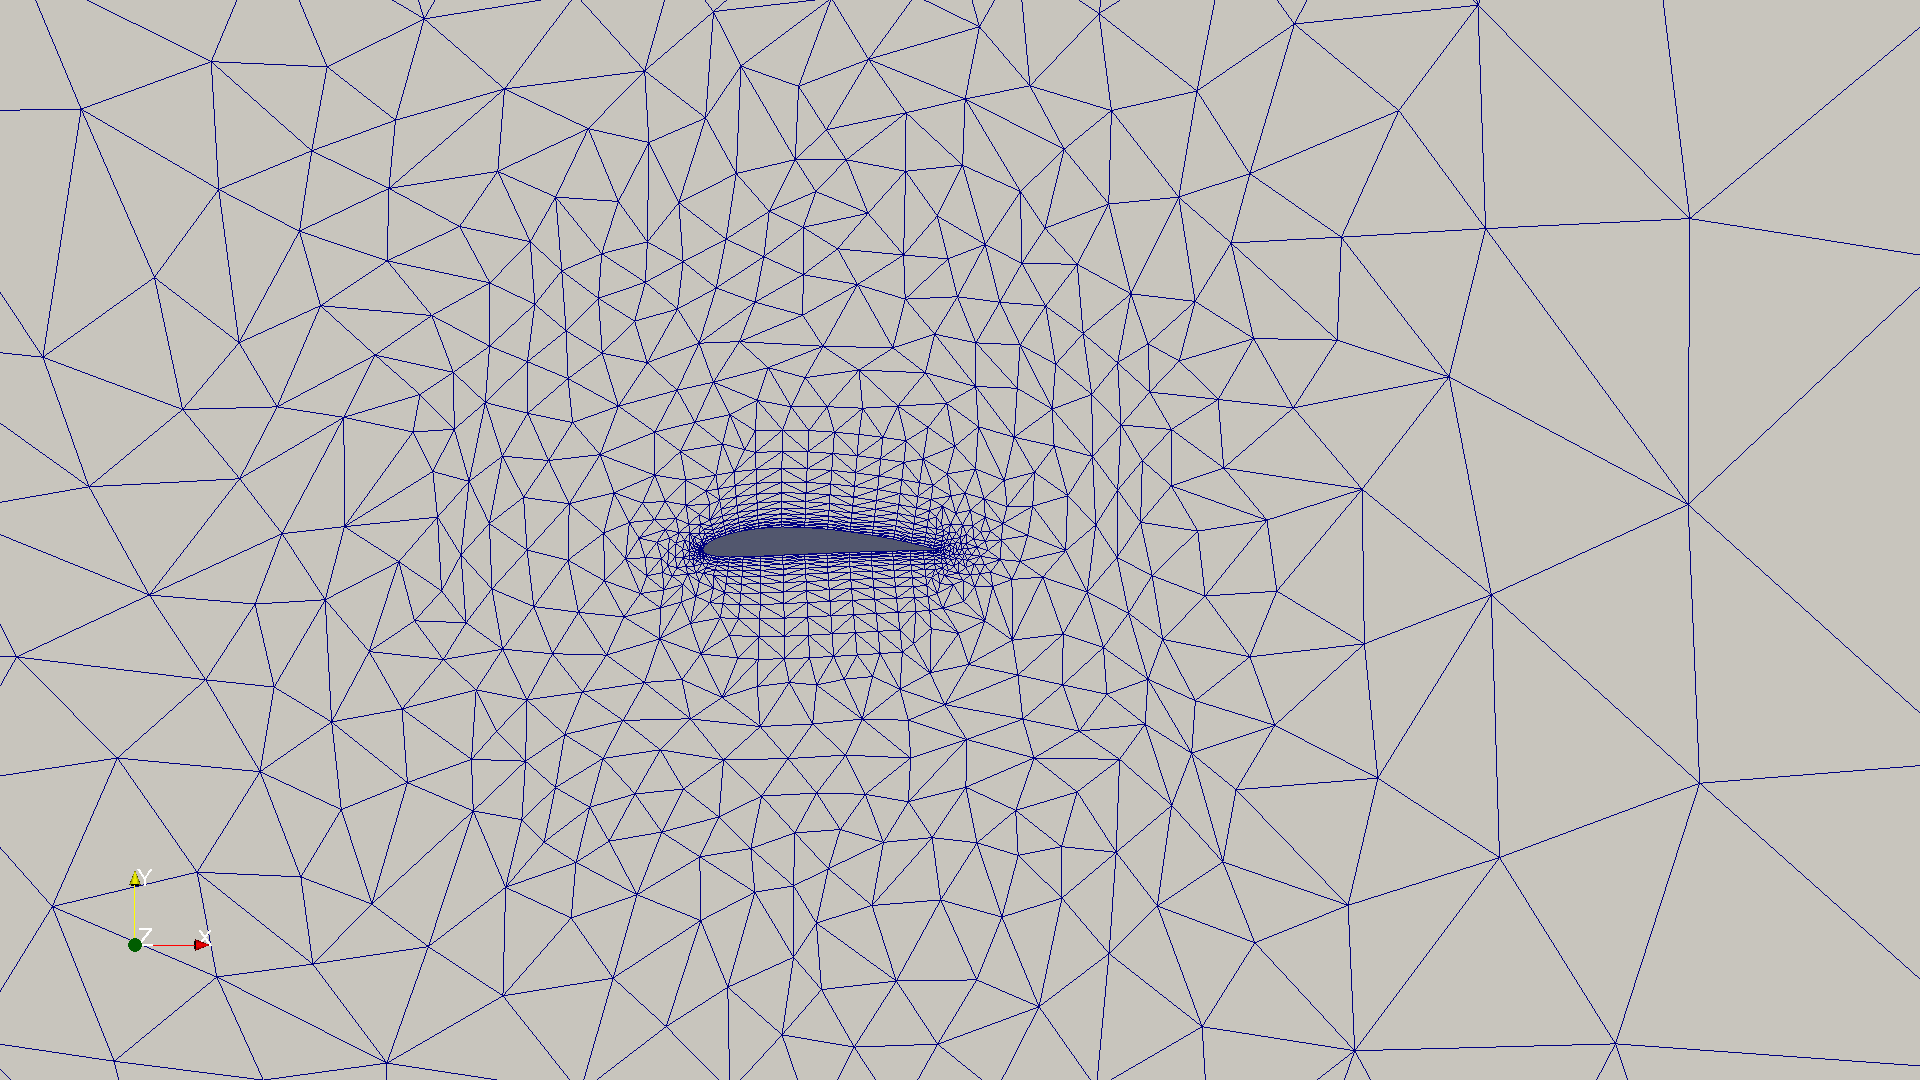
\includegraphics[width=0.18\textwidth,trim={0 0 0 0},clip]{mesh_5p5k_2.png}
\hspace*{1mm}
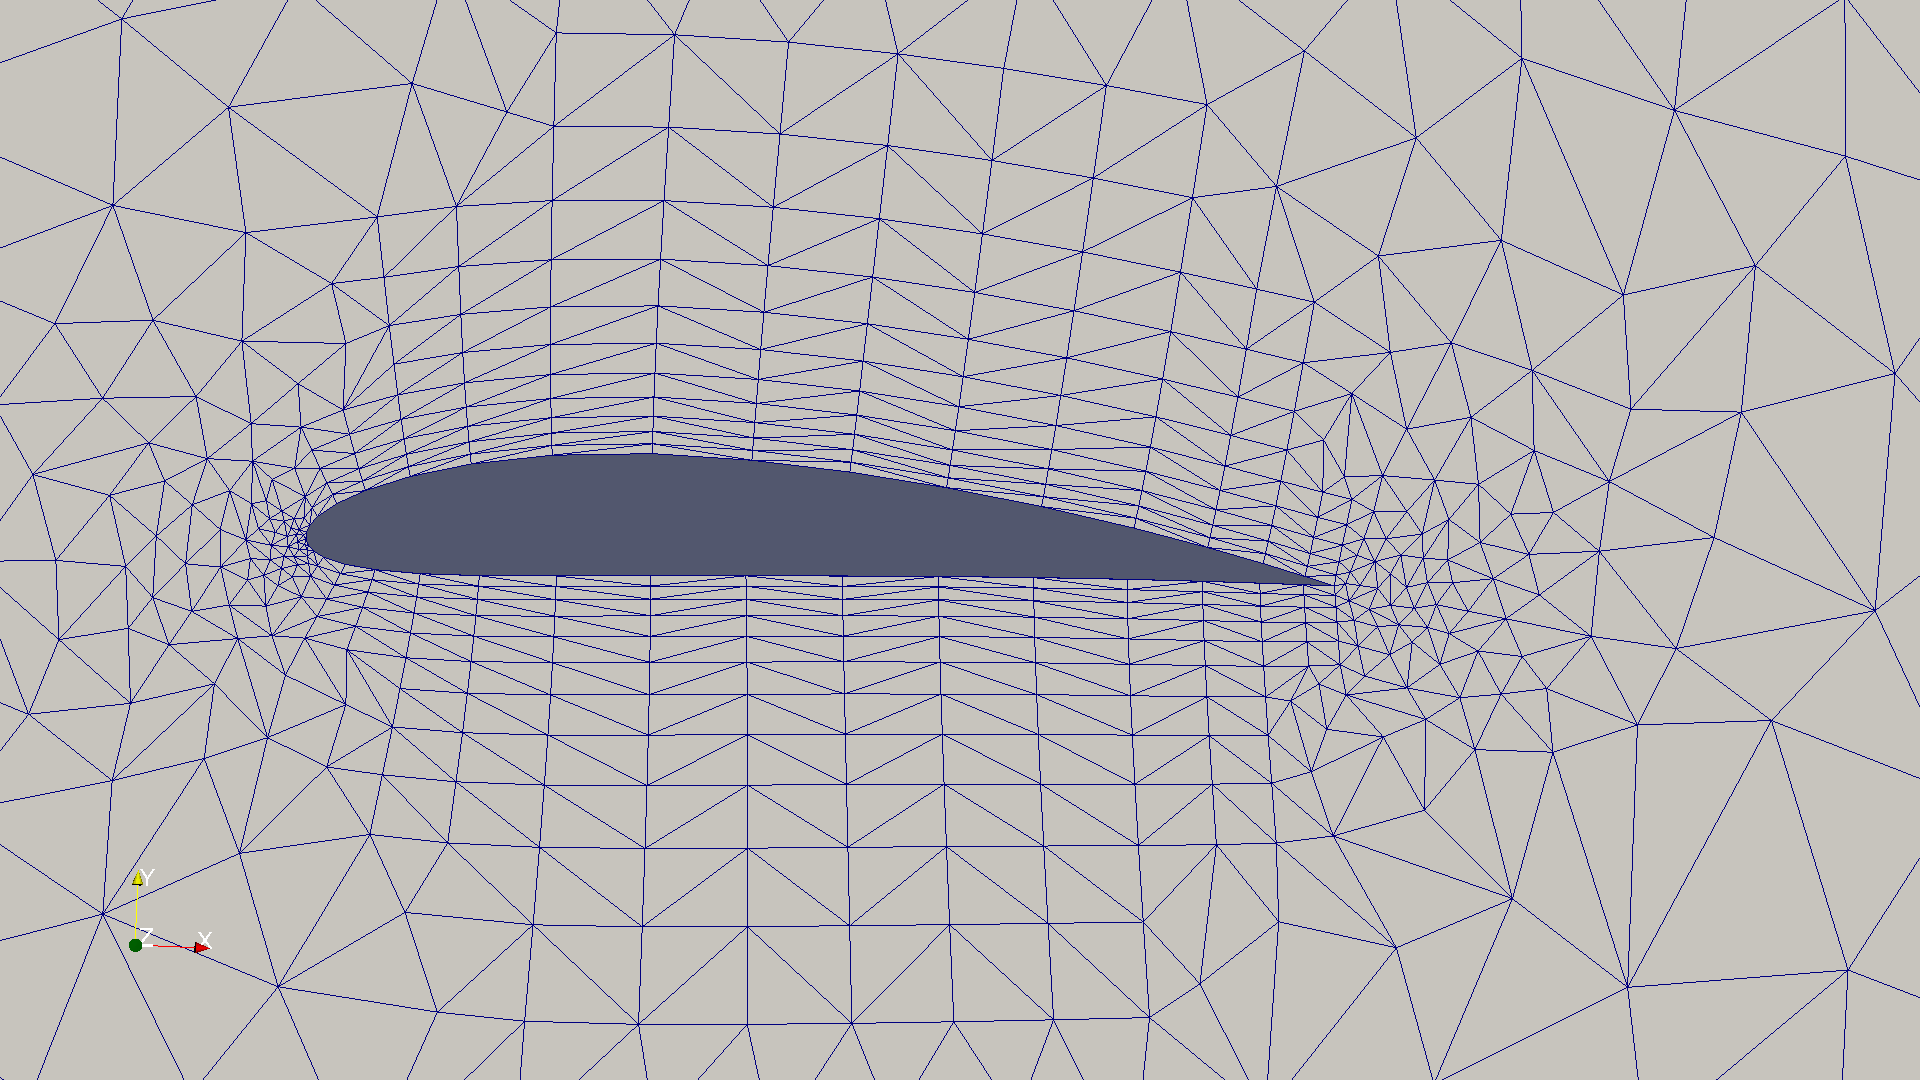
\includegraphics[width=0.18\textwidth,trim={0 0 0 0},clip]{mesh_5p5k_3.png}
\hspace*{1mm}
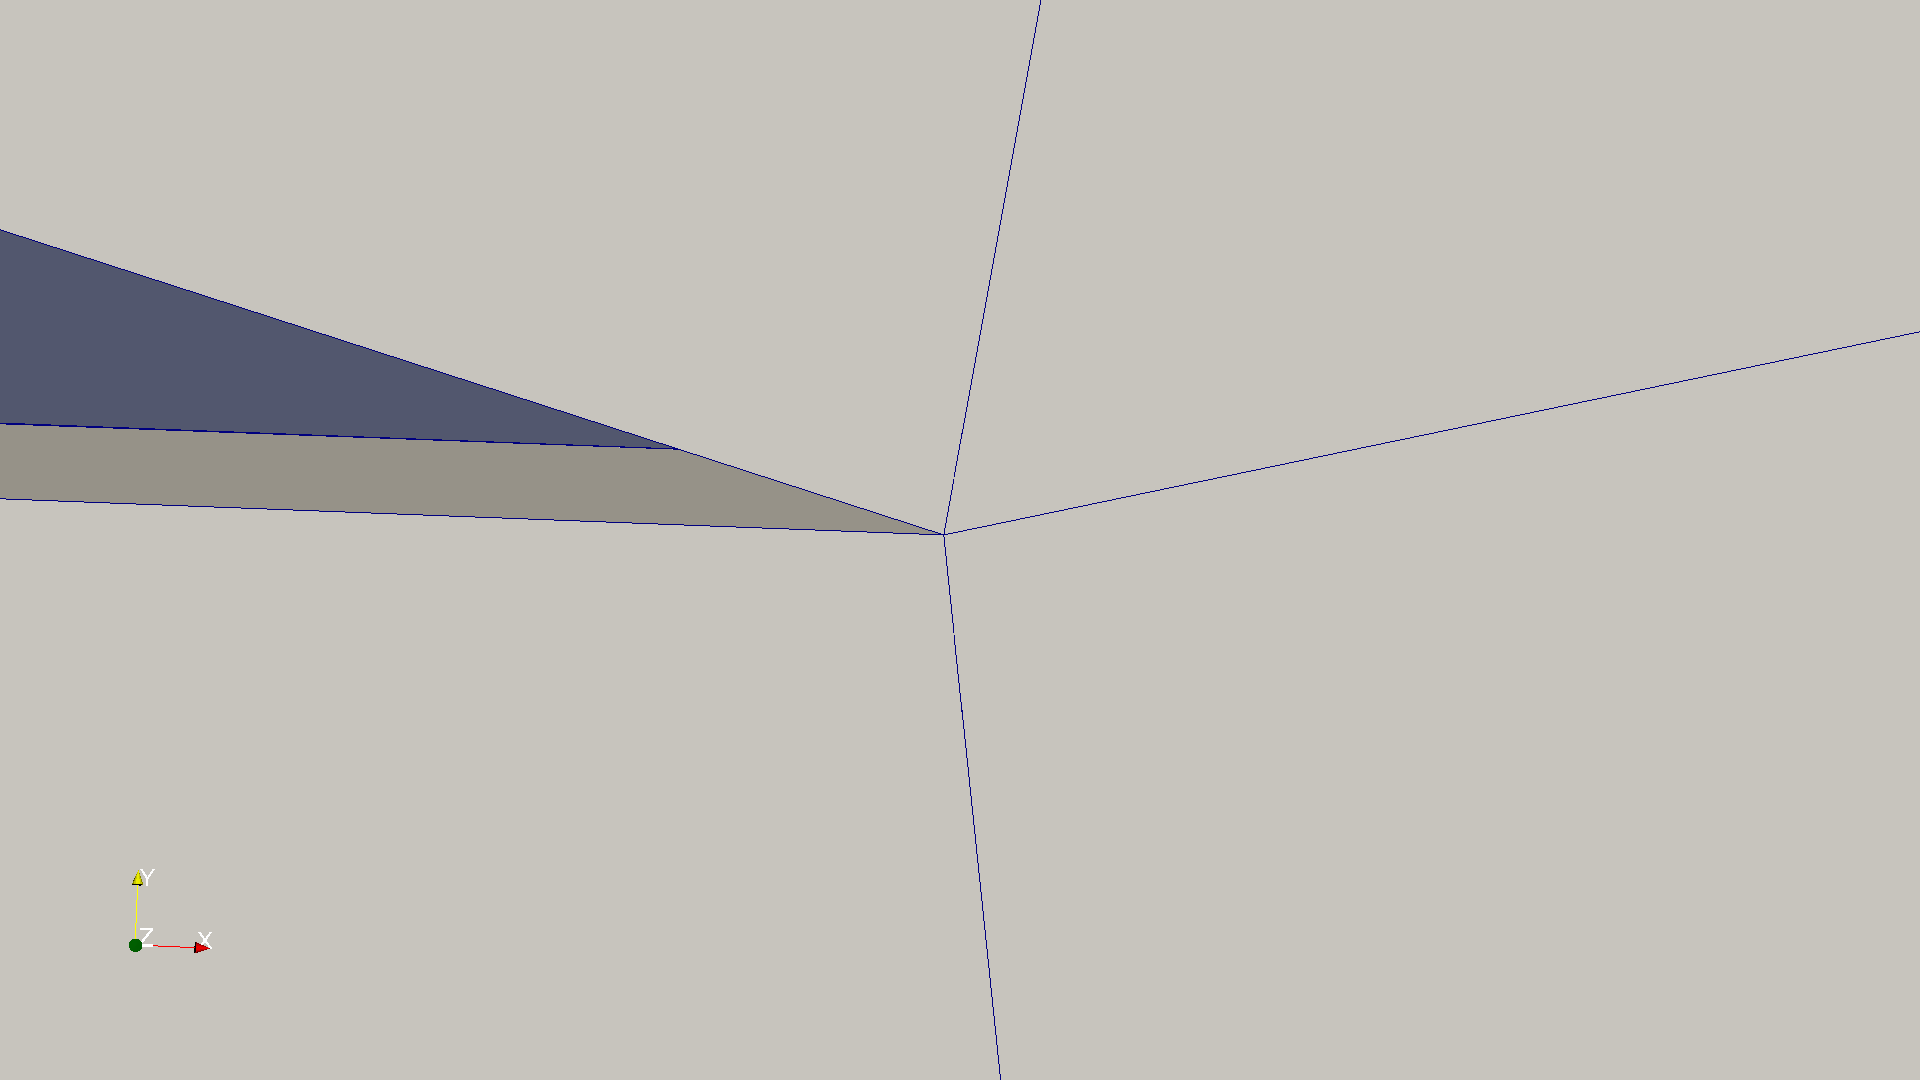
\includegraphics[width=0.18\textwidth,trim={0 0 0 0},clip]{mesh_5p5k_4.png}
\\[3mm]
\begin{overpic}[width=0.4\textwidth,trim={0 377px 0 377px},clip]{mesh_32k_1.png}
	\put (0,19) {Fine: 32,000 tetrahedral elements}
\end{overpic}
\hspace*{1mm}
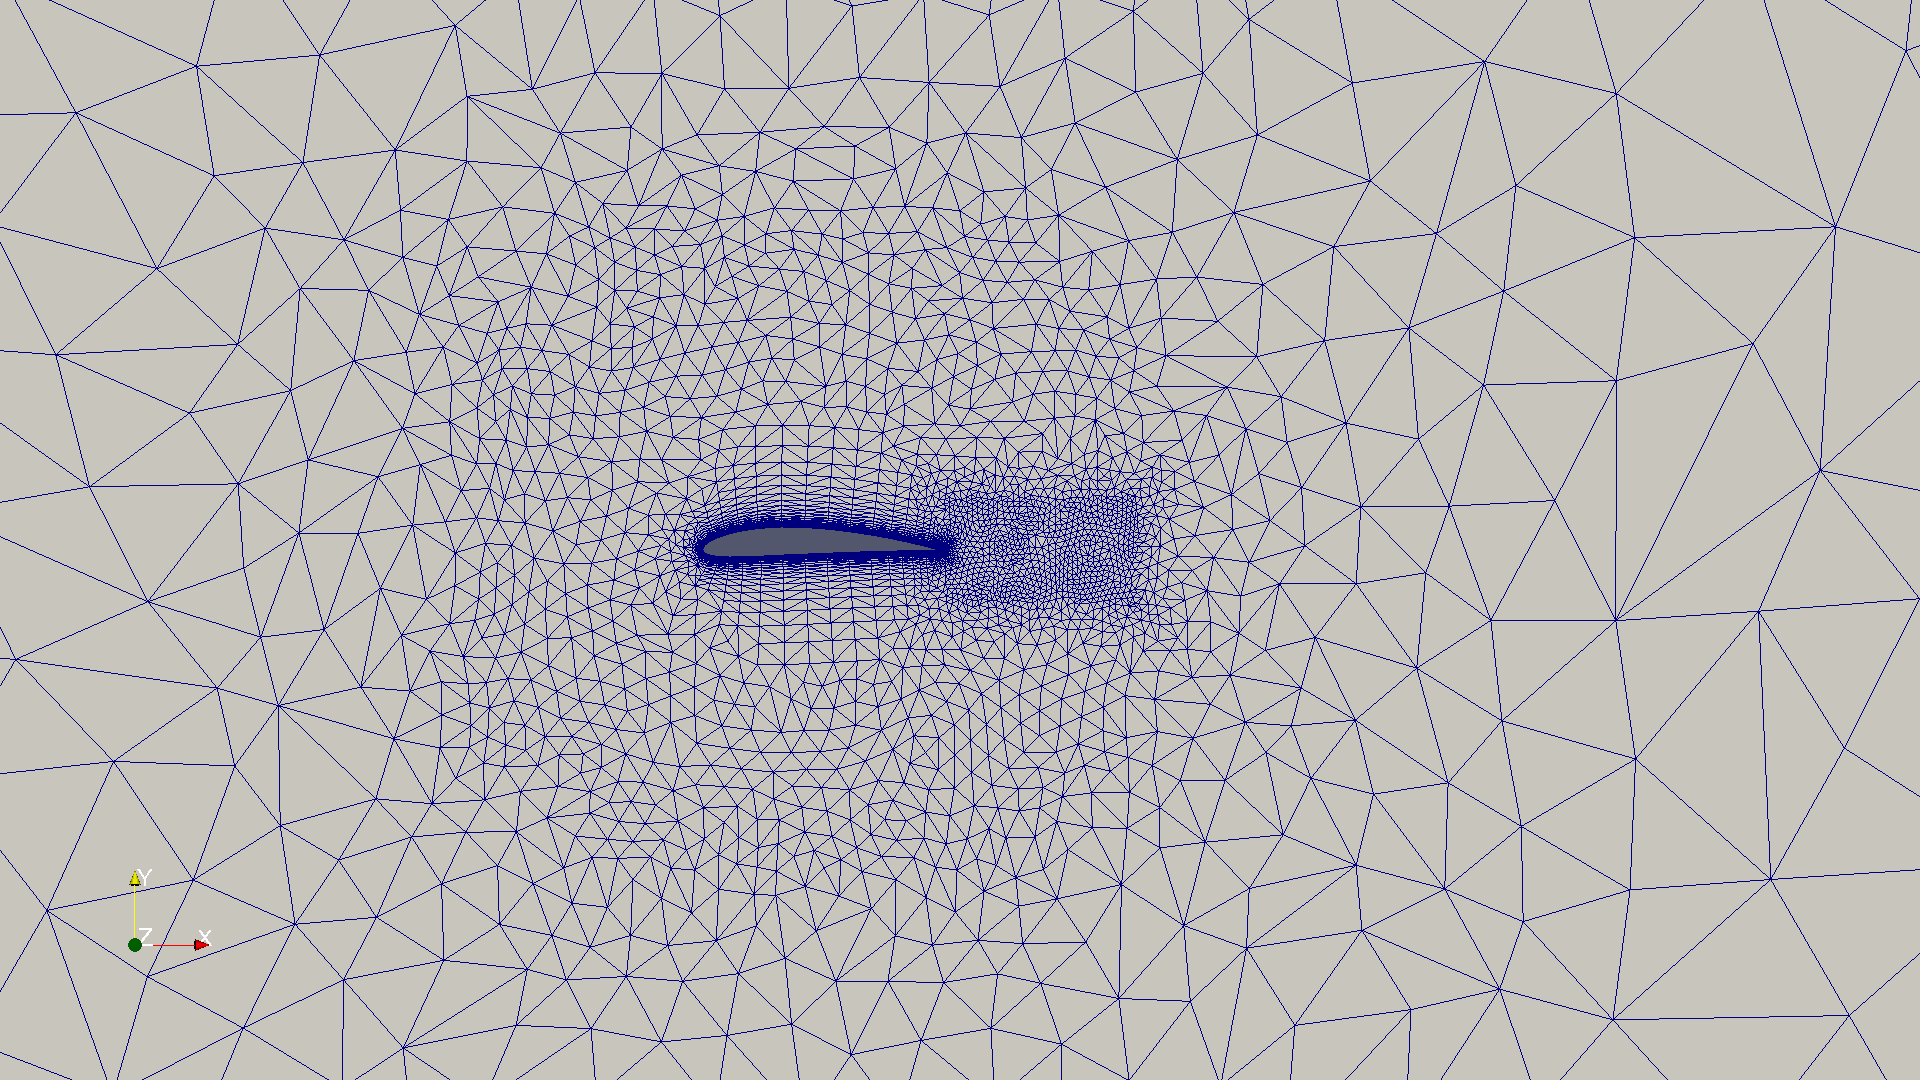
\includegraphics[width=0.18\textwidth,trim={0 0 0 0},clip]{mesh_32k_2.png}
\hspace*{1mm}
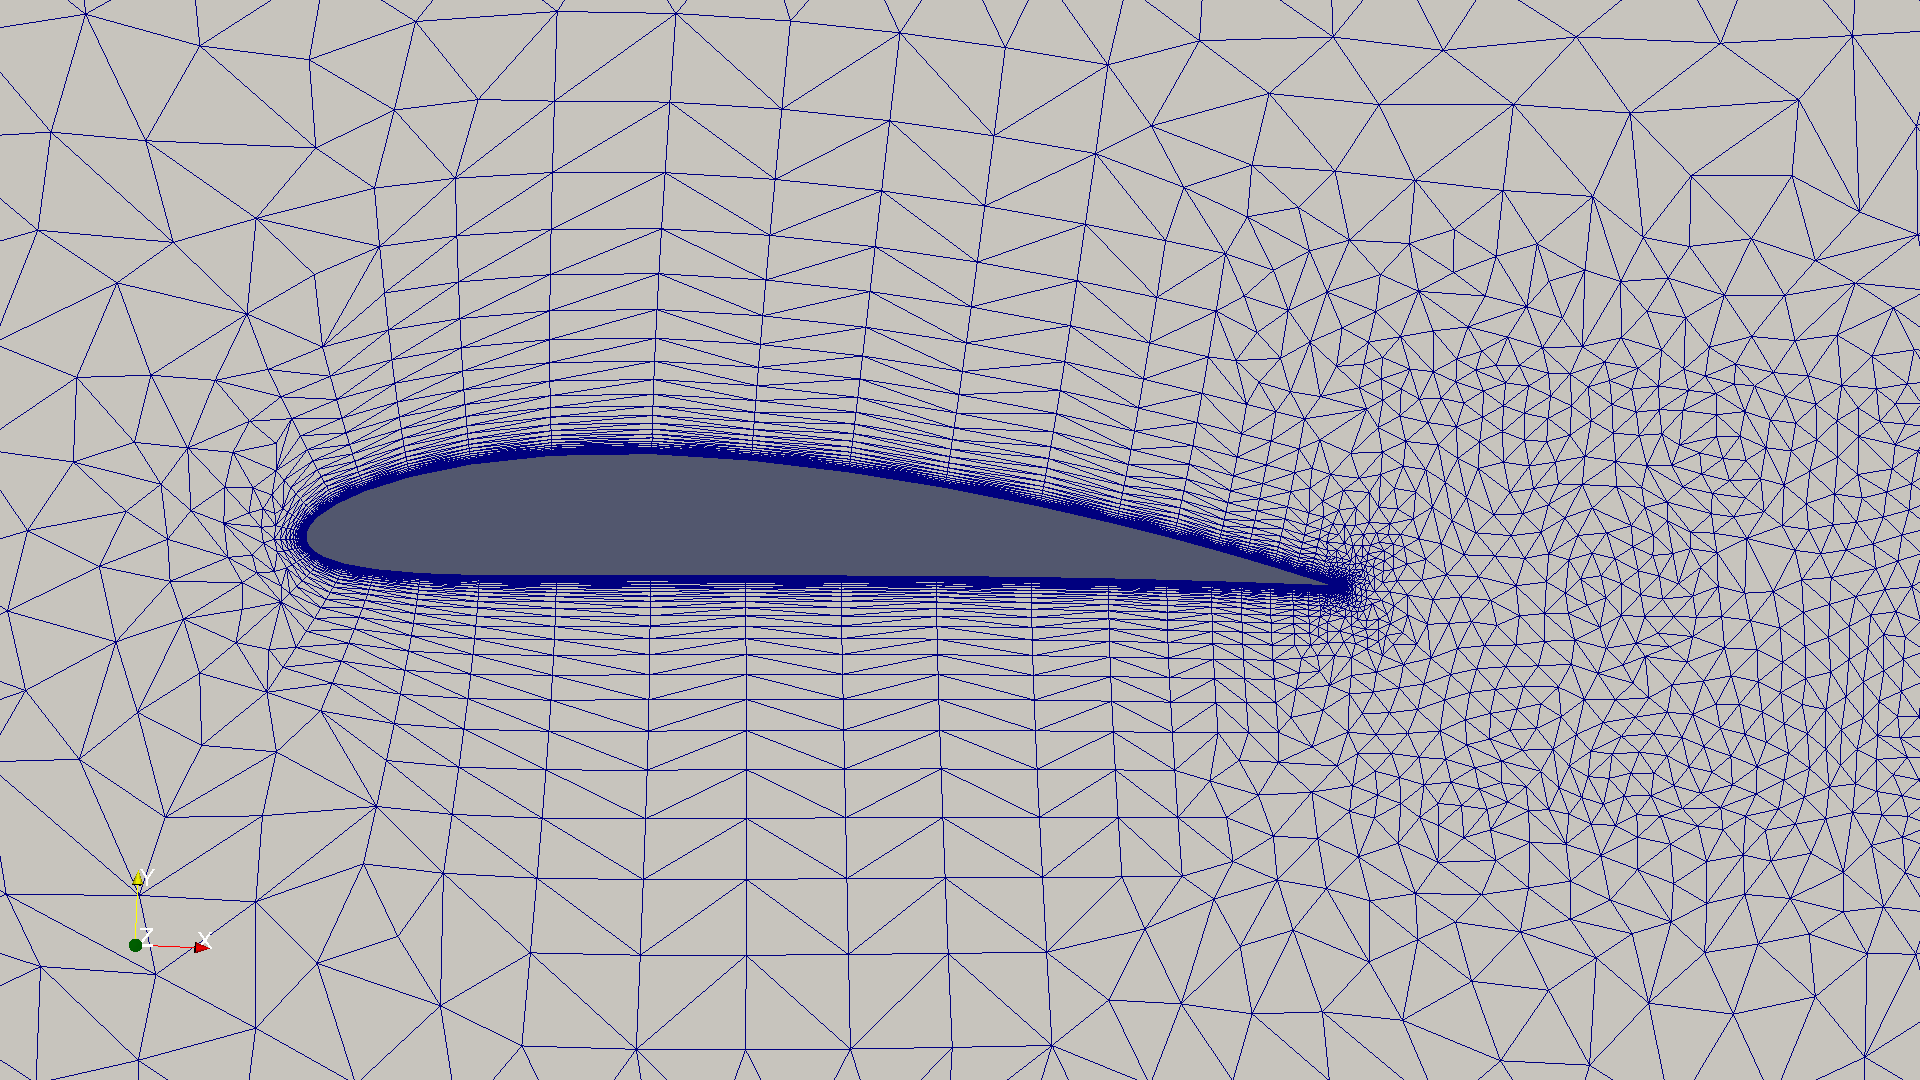
\includegraphics[width=0.18\textwidth,trim={0 0 0 0},clip]{mesh_32k_3.png}
\hspace*{1mm}
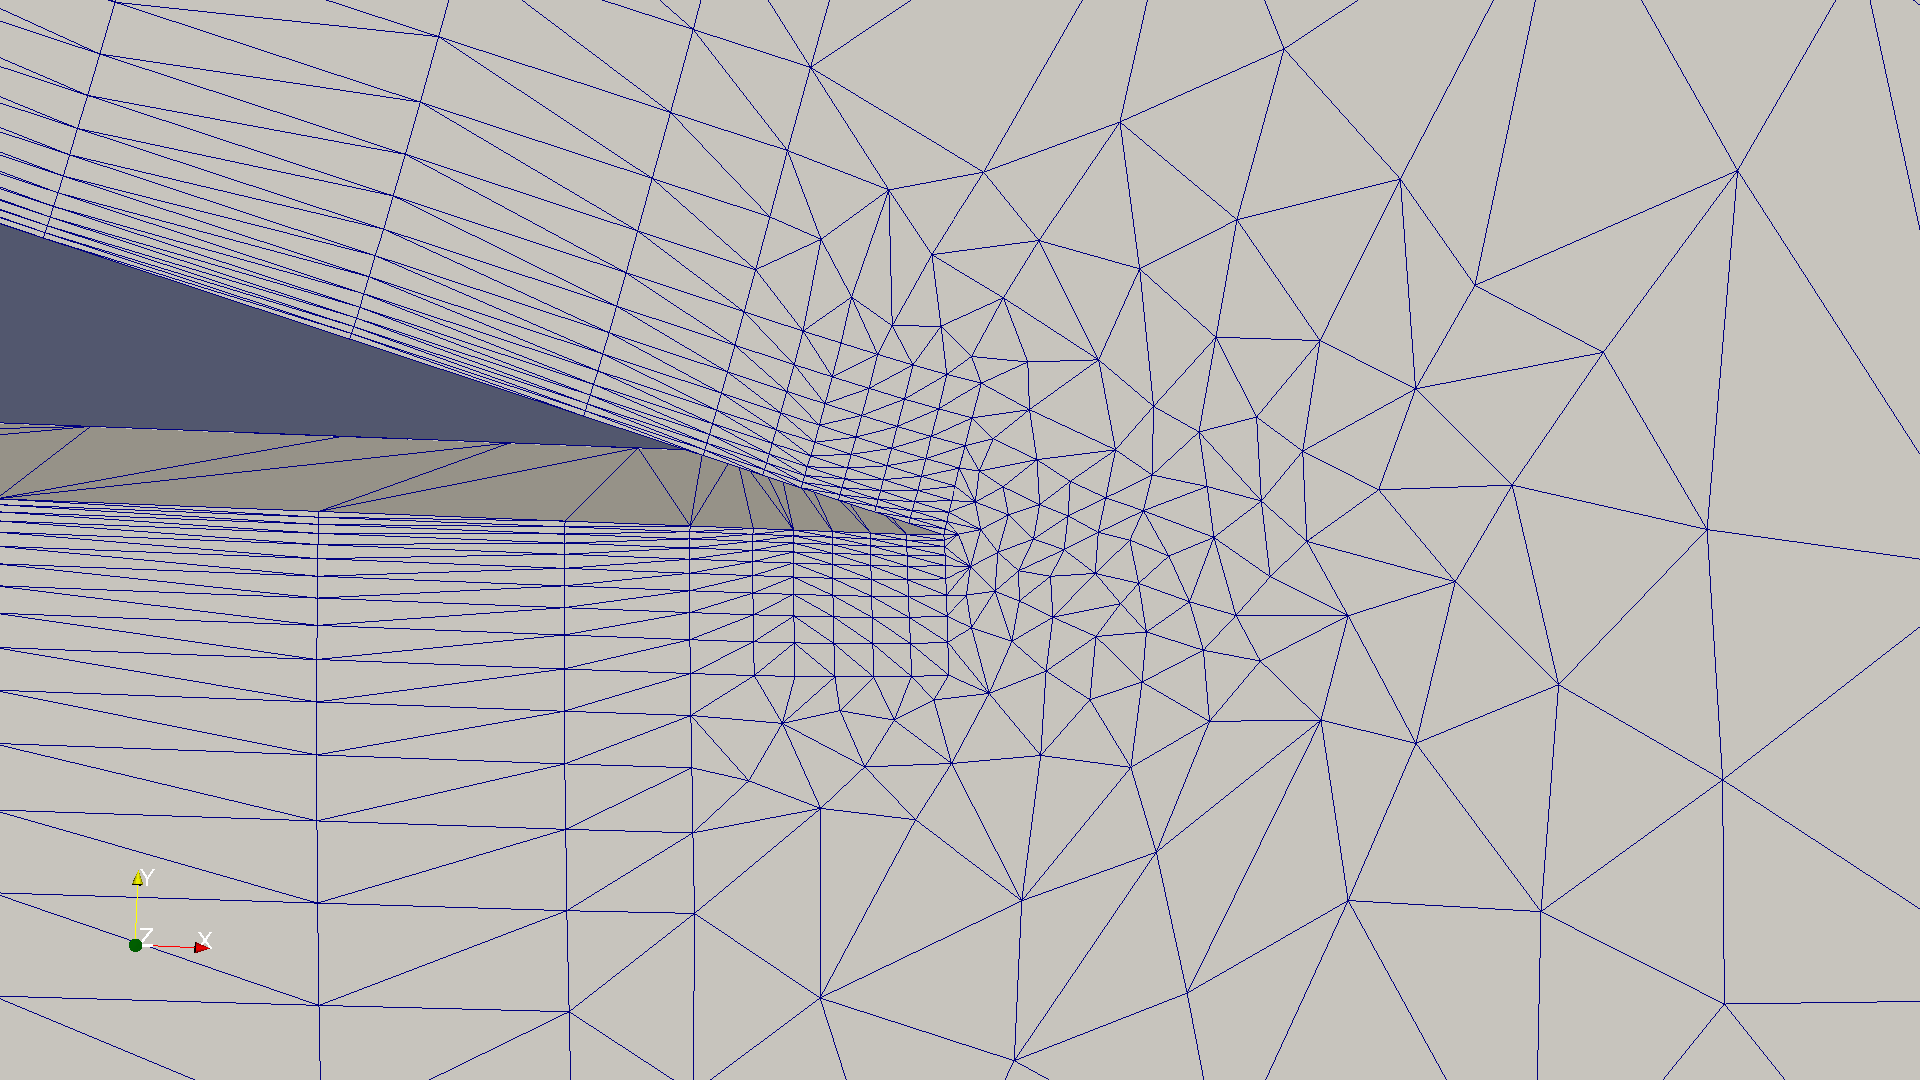
\includegraphics[width=0.18\textwidth,trim={0 0 0 0},clip]{mesh_32k_4.png}
\\[2ex]
\caption{Coarse (top) and fine (bottom) 2-D mesh of fluid domain around a NACA 4412 airfoil. Left to right: zooming in from full domain to trailing edge of airfoil. Note the lack of shear layer and near-wall resolution on coarse mesh.}
\label{fig:mesh_coarse}
\end{center}
\end{figure}

The converged NACA 0012 flow solution acts as the starting point for each new combination of geometric parameters we want to test. This means we skip the start-up transient of ``turning on'' the simulated wind tunnel for subsequent geometries, resulting in efficiency gains. Geometric parameters are specified in an ASCII input file. Upon reading this file, PHASTA applies a displacement to each node on the surface of the airfoil, represented by the black lines in Figure \ref{fig:naca_deform}. A linear elastic structural solver\footnote{Courtesy of Eric Peters, University of Colorado at Boulder} satisfies the displacement constraints and deforms the entire mesh in accordance with the specified geometric parameters. Positive volumes on BL elements are preserved by enforcing an inverse relationship between element volume and stiffness. As before, numerical solution of the flow equations proceeds until statistically-steady results are obtained.

\subsection{Interpolating Decomposition and Runs Conducted}

Three sets of random geometric parameters used, corresponding to cases 1, 2, and 3 in Table \ref{tbl:rand_params}. For a given case, we represent them as the stochastic vector 
\begin{equation}
\bm{y} = \begin{bmatrix}
\bm{m} & \bm{p} & \bm{t} & \bm{c} & \bm{\alpha}
\end{bmatrix}^T
\end{equation}
When an individual run meets the stopping criterion described above, $C_p$ information is extracted from the solution file through a ParaView script, and stored with an identifier linking the run to its specific realization of geometric parameters.

\begin{table}[t]
\begin{center}
\begin{tabular}{@{}llllll@{}}
\toprule
Case & $\bm{m}$ & $\bm{p}$ & $\bm{t}$ & $\bm{c}$ & $\bm{\alpha}$ \\
\midrule
1 & $U[0,0.1]$ & $U[0.3,0.6]$ & $U[0.05,0.2]$ & $1.0$ & $U[0,7]$ \\
2 & $U[0.045,0.055]$ & $U[0.3825,0.5175]$ & $U[0.1156,0.1344]$ & $1.0$ & $U[0,7]$ \\
3 & $0.04$ & $0.4$ & $0.12$ & $1.0$ & $U[-2,2]$ \\
\bottomrule
\end{tabular}
\end{center}
\caption{Geometric random variables used in each of the three cases. (1) arbitrary ranges for initial study, (2) arbitrarily defined ``manufacturing error'' for geometric parameters at variable $\bm{\alpha}$, (3) NACA 4412 airfoil with small variation in $\bm{\alpha}$ to crudely model atmospheric turbulence.}
\label{tbl:rand_params}
\end{table}

Each realization of random parameters is denoted by $\bm{y}^{(i)}$, where $i = 1, \dots, K$. The values of $C_p$ at all $m$ points on the airfoil surface are collected in a solution vector $\bm{u}(\bm{y}^{(i)})$ for each geometric realization $i$. LF and HF solutions are denoted by a superscript, respectively $\bm{u}^L(\bm{y}^{(i)})$ and $\bm{u}^H(\bm{y}^{(i)})$.

The set of $K$ LF solutions are collected into a matrix
\begin{equation}
\bm{U}^L
\equiv
\begin{bmatrix}
\vline & \vline & & \vline \\
\bm{u}^L(\bm{y}^{(1)}) & \bm{u}^L(\bm{y}^{(2)}) & \cdots & \bm{u}^L(\bm{y}^{(K)}) \\
\vline & \vline & & \vline
\end{bmatrix}_{m \times K}
\end{equation}
where each column holds a single LF solution vector. An interpolating decomposition \citeme (ID) constructs a rank-$r$ approximation to $\bm{U}^L$ as the product of a column skeleton matrix $\bm{U}^L_C$ and the coefficient matrix $\bm{\Lambda}^L$.
\begin{equation}
\begin{aligned}
\bm{U}^L
&\approx
\begin{bmatrix}
\vline & \vline & & \vline \\
\bm{u}^L(\bm{y}^{(1)}) & \bm{u}^L(\bm{y}^{(2)}) & \cdots & \bm{u}^L(\bm{y}^{(r)}) \\
\vline & \vline & & \vline
\end{bmatrix}_{m \times r}
\begin{bmatrix}
\lambda^L_{ij}
\end{bmatrix}_{r \times K}
\\
&= \bm{U}^L_C \bm{\Lambda}^L
\end{aligned}
\end{equation}
It is important to note that the $r \ll K$ basis vectors selected to decompose the full-rank $\bm{U}^L$ matrix are taken from that matrix itself. Thus, the columns of $\bm{U}^L_C$ correspond to specific realizations of $\bm{y}$. Furthermore, the decomposition rank $r$ is not fixed; it can be varied depending on the desired accuracy of the ID.

To compute the bi-fidelity model, we first obtain high-fidelity solutions corresponding the geometric realizations deemed important by the LF ID. These populate a HF column skeleton $\bm{U}^H_C$. Then we reverse the ID to calculate our approximation $\hat{\bm{U}}^H$ of $K$ HF solutions,
\begin{equation}
\begin{aligned}
\hat{\bm{U}}^H
&=
\begin{bmatrix}
\vline & \vline & & \vline \\
\bm{u}^H(\bm{y}^{(1)}) & \bm{u}^H(\bm{y}^{(2)}) & \cdots & \bm{u}^H(\bm{y}^{(r)}) \\
\vline & \vline & & \vline
\end{bmatrix}_{m \times r}
\begin{bmatrix}
\lambda^L_{ij}
\end{bmatrix}_{r \times K}
\\
&= \bm{U}^H_C \bm{\Lambda}^L
\end{aligned}
\end{equation}

For each case in Table \ref{tbl:rand_params}, $K=1000$ LF and 1000 HF runs are conducted. The ID and corresponding bi-fidelity model are both computed for different $r$. The ID and bi-fidelity model's error relative to the LF and HF runs, respectively, are computed using the Frobenius matrix norm,
\begin{equation}
\| \bm{M} \|_\text{Fro} \equiv \sqrt{\sum_i \sum_j M_{ij}^2}
\end{equation}

%%%%%%%%%%%%%%%%%%%%%%%%%%%%%%%%%%%%%%%%%
%%%%%%%%%%%%%%%%%%%%%%%%%%%%%%%%%%%%%%%%%
\section{Results}
%%%%%%%%%%%%%%%%%%%%%%%%%%%%%%%%%%%%%%%%%
%%%%%%%%%%%%%%%%%%%%%%%%%%%%%%%%%%%%%%%%%


\section{Conclusion and Discussion}


%%
%% DOCUMENT END
%%
\label{lastpage}
\end{document}



























